 Deep Learning is part of machine learning methods based on artificial neural networks. %with representation learning. %Learning can be supervised, semi-supervised or unsupervised. 
 Part of the theoretical basis underlying Deep Learning  initially emerged as models for understanding the human learning process, that is, how the brain works. Thus, these theories are related with Deep Learning  that has grown the most in recent years \cite{goodfellow2016}.

Deep learning methods have achieved excellent performance over traditional machine learning methods, mainly due to the development of the area, but also by the increase in computational power and the amount of available data \cite{geron2019}. 

Computer vision is a field that has been using Artificial Intelligence (AI) extensively, as it also seeks to reproduce some of the human capabilities in autonomous systems. The main aim of computer vision is to make computers perform functions similar to human vision, being able to receive visual data and perform its processing. The performance improvement in computer vision is strongly related with the evolution of machine learning.

Traditional computer vision techniques were almost entirely pipelined by hand, where the features to be extracted and the algorithms used were done manually. This made such techniques more difficult to adapt to different tasks. With the emergence of deep learning, it became possible to use these networks to perform this feature extraction work, in addition to the algorithm part, where machine learn performs the task.

\begin{figure}
    \centering
    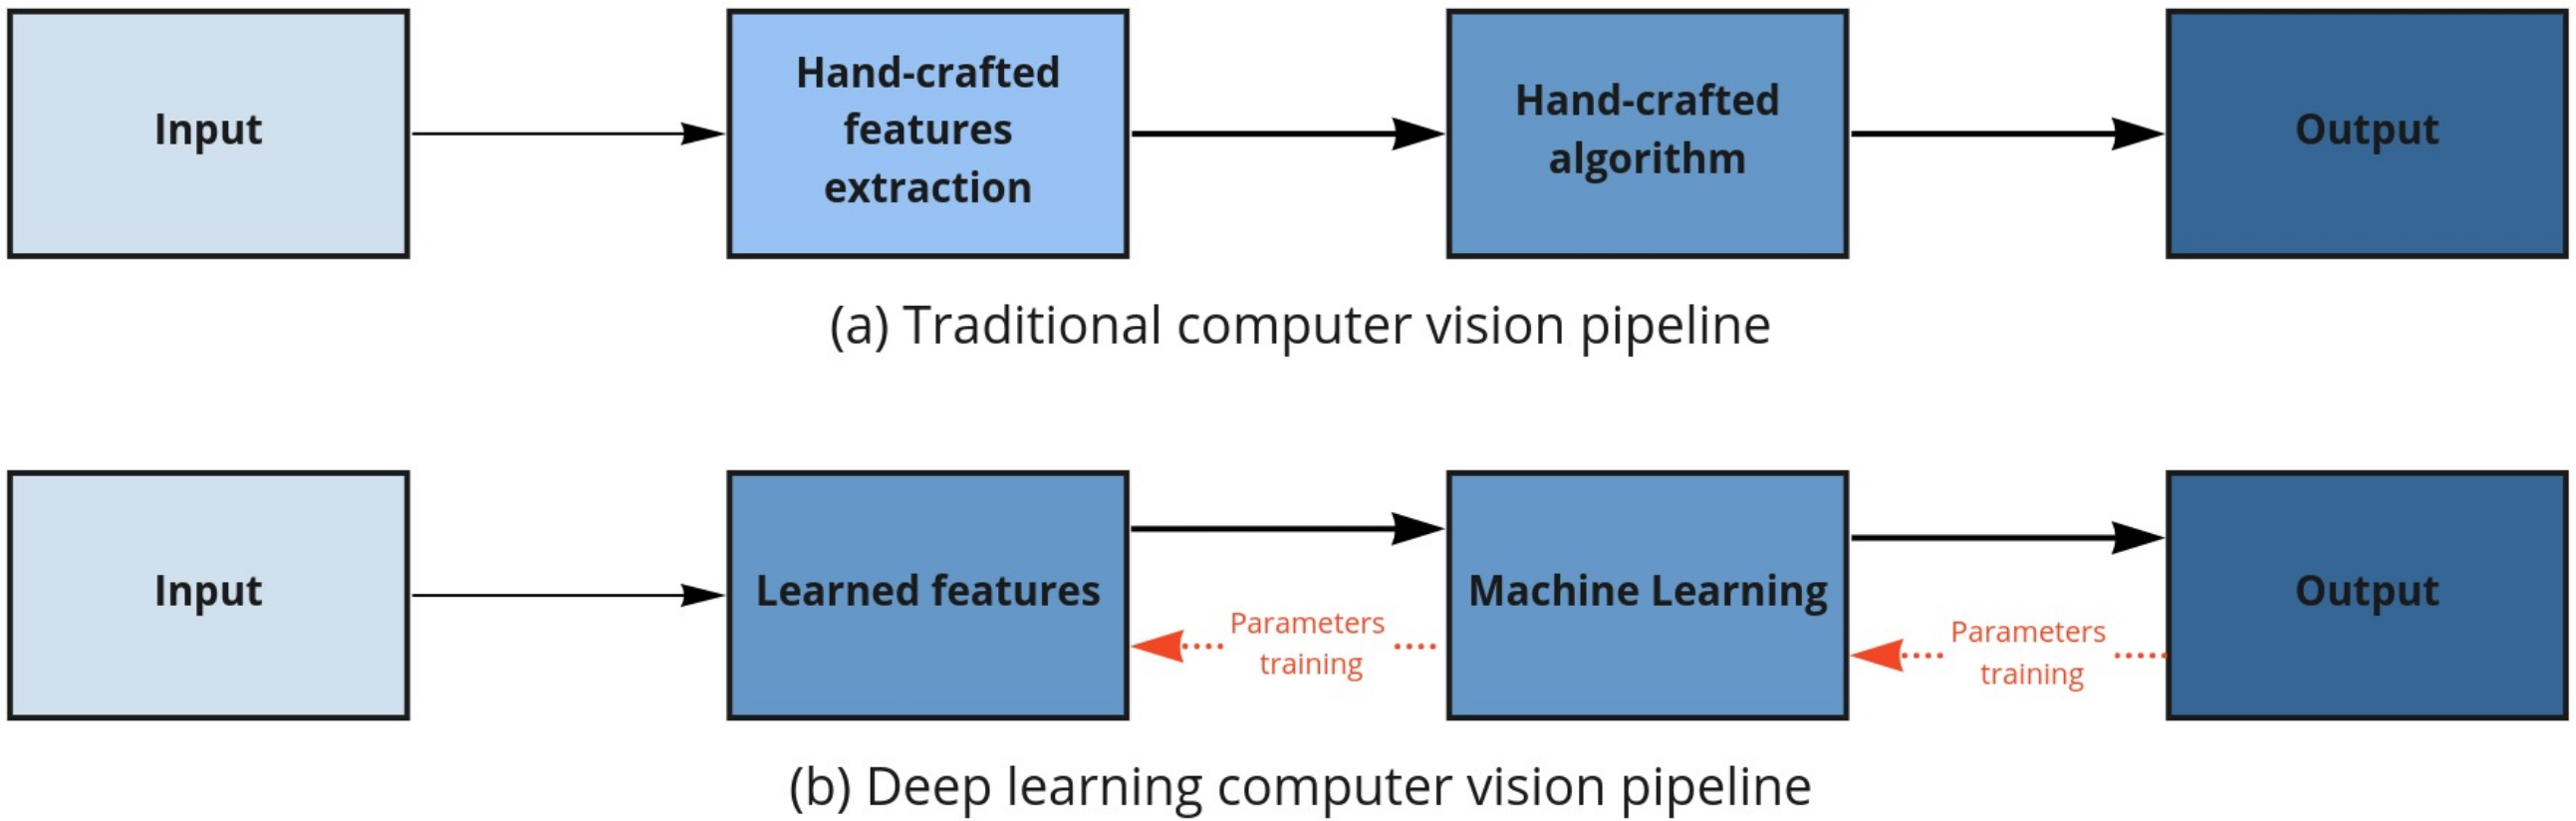
\includegraphics[scale=0.20]{"Part 3 - Learning Systems/Supervised Learning/Deep Learning/images/cvpipeline.png"}
    \caption{Traditional(a) and Deep learnign(b) computer vision pipelines. Inspired in \cite{szeliski2010computer}(Figure 5.2)}
    \label{fig:figurecvpipeline}
\end{figure}

Figure \ref{fig:figurecvpipeline} presents two preprocessing scenarios. The traditional(\ref{fig:figurecvpipeline} (a)), where the two principal steps, the selection of features to be extracted and the algorithm that uses these features, are mannually adjusted. The Deep learning pipeline(\ref{fig:figurecvpipeline} (b)), where the model learns which features to extract and how use these features to get the desired output. The red arrow in the Deep Learning pipeline shows how this type of model uses information about the output to adjust the parameters of the network, and consequently, learns a problem.

Among the many deep learning architectures, the Convolutional Neural Networks (CNN) is one of the most widely used as it is very similar to a conventional MLP.

\section{Convolutional Neural Networks (CNN)}

Conventional neural networks are, basically, formed by neurons and connections between them to build a model. Convolutional neural networks, on the other hand, have some more structures, which are the reason for their better performance in handling images. We will see them next.


\subsection{Convolution Layers}

The operation that gives name to this artificial neural network, the convolution, is an operation performed between two functions. In the case, as the operation is performed with images, discrete convolution is used.

%An important point to note is that mathematically what we will call a convolution is actually a correlation, and the two are almost identical, except for the fact that in the convolution we rotate the filter (kernel) by 180\textdegree . The only advantage we gain from turning the filter before the operation is that we gain the commutative property, which is mathematically useful for proof derivation but not important in Deep Learning  implementation \cite{goodfellow2016}.

In Deep Learning  literature and libraries, it has become common to call correlation as convolution \cite{goodfellow2016}, so we will also use this convention, using convolution without rotating the filter, so a correlation.
The discrete correlation formula is given by Equation \ref{correlation}:

\begin{equation}
\label{correlation}
g(x,y)=w(x,y)\star f(x,y)=\sum_{s=-a}^a\sum_{t=-b}^bw(s,t)f(x+s,y+t)
\end{equation}

\noindent Where $\star$ represents the correlation operation; $w$ consists in a filter (kernel), a matrix of numbers, usually with odd square size (to facilitate operations), and $f$ an image in a matrix format. And related to this is the formula of convolution ($g$):

\begin{equation}
g(x,y)=w(x,y)\ast f(x,y)=\sum_{s=-a}^a\sum_{t=-b}^bw(s,t)f(x-s,y-t)
\end{equation}

As can be seen by looking at the two equations, these operations are very simple, being basically a summation of products. Figure \ref{fig:figure117} presents the correlation step where the following operation takes place:

%corrigir orientação
\begin{equation}
\begin{split}
w*f(0,0)=\sum_{s=1}^{2}\sum_{t=1}^{2}w(s,t){f}(0-s,0-t)= \\
w(0,0)f(0,0)+w(0,1)f(0,1)+w(0,2)f(0,2) \\
+w(1,0)f(1,0)+w(1,1)f(1,1)+w(1,2)f(1,2) \\
+w(2,0)f(2,0)+w(2,1)f(2,1)+w(2,2)f(2,2)\\
=(-1)\cdot5+(-2)\cdot7+(-1)\cdot0\\
+0\cdot6+0\cdot0+0\cdot1\\
+1\cdot6+2\cdot2+1\cdot2
=-19-0+12=-7
\end{split}
\end{equation}

\begin{figure}
    \centering
    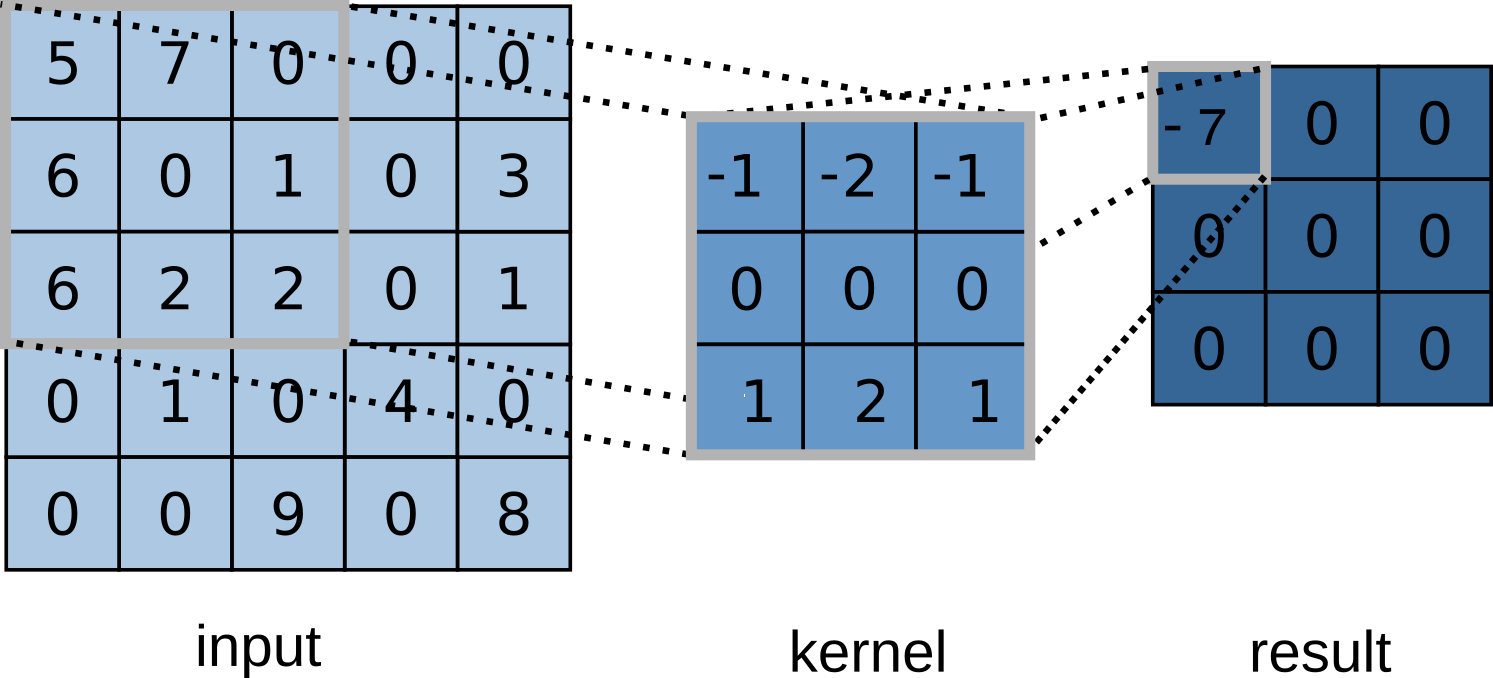
\includegraphics[scale=0.40]{"Part 3 - Learning Systems/Supervised Learning/Deep Learning/images/figure117.png"}
    \caption{Convolution of a 5x5 sized image with a 3x3 sized kernel and its result.}
    \label{fig:figure117}
\end{figure}

Figure \ref{fig:figure117} depicts an illustration of the convolution operation, however, in real world applications the input image is represented by a simple matrix (configuring a grayscale image) but most of the time images that contain three dimensions are used. In this case, there is an image in the RGB model, where three matrices will be present, each one representing a color channel. Figure \ref{fig:figure118} depicts an example of convolution for an RGB image. There is a kernel also made up of three matrices. An important thing to note is that the number of layers in the input filter has to be equal to the number of channels in the image for the convolution operation to be done.

\begin{figure}
    \centering
    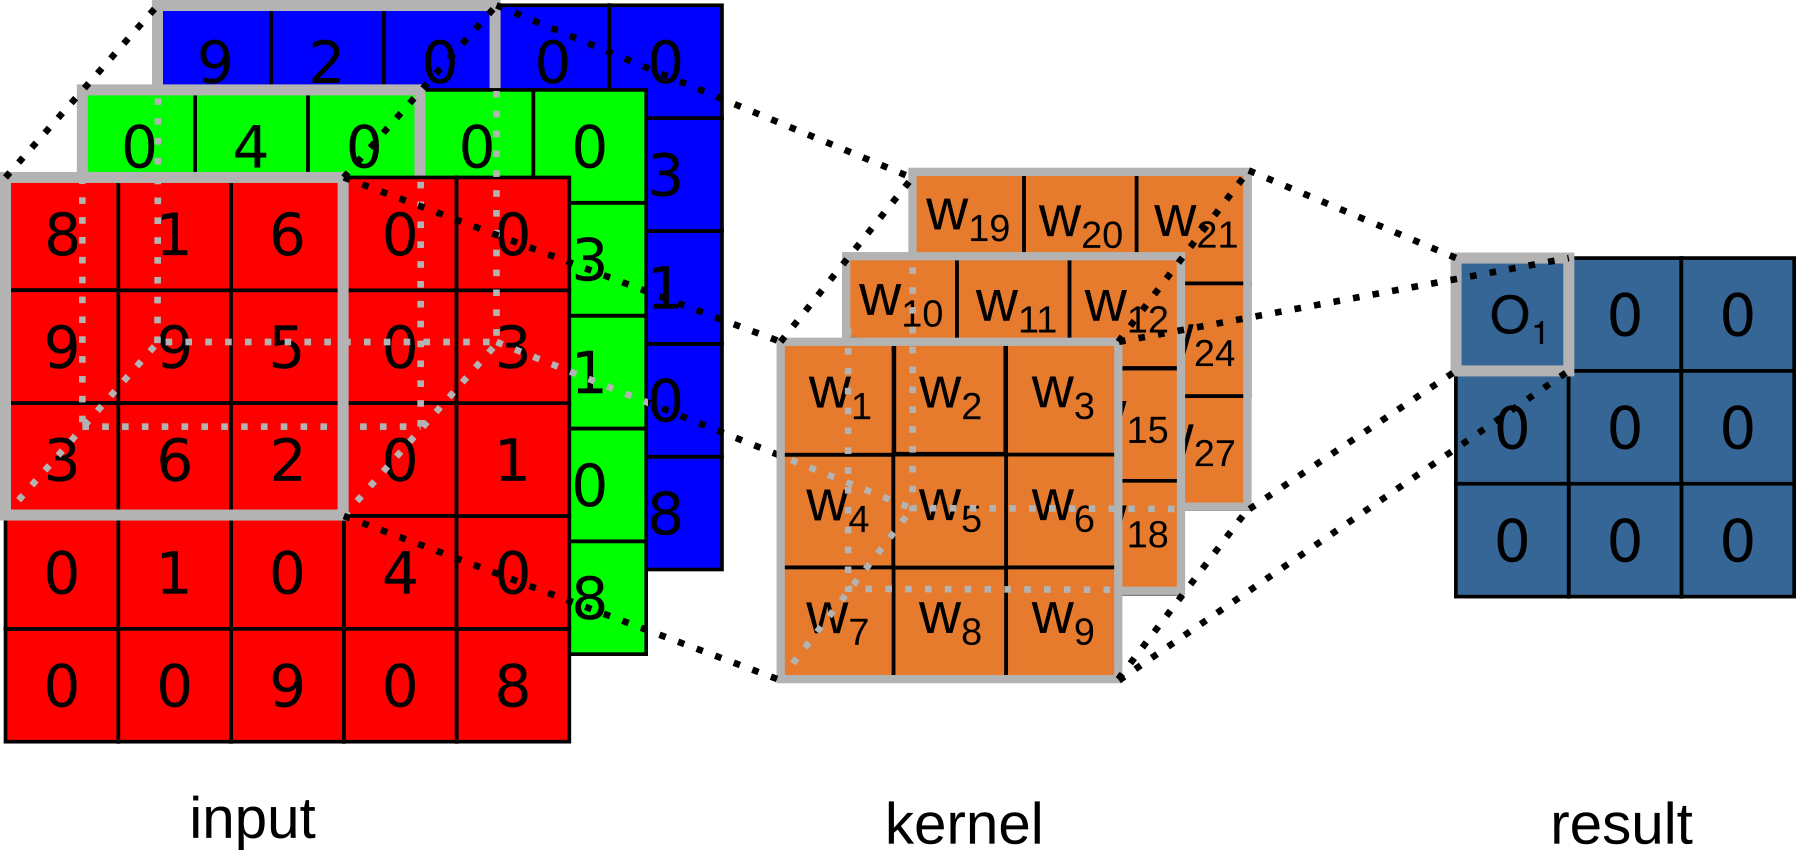
\includegraphics[scale=0.35]{"Part 3 - Learning Systems/Supervised Learning/Deep Learning/images/figure118.png"}
    \caption{Convolution of a 5x5x3 sized image with a 3x3x3 sized kernel and its result.} 
    \label{fig:figure118}
\end{figure}

Figure \ref{fig:figure119} depicts a representation of a convolution layer with more than one filter. For each filter, there is an output matrix and, consequently, as a final result a dataset where the number of depth layers (also known as feature map, illustrated by the three matrices in orange) will correspond to the number of filters applied to the input. This output can then be sent forward on the network, going through more convolutions and having more features extracted.

\begin{figure}
    \centering
    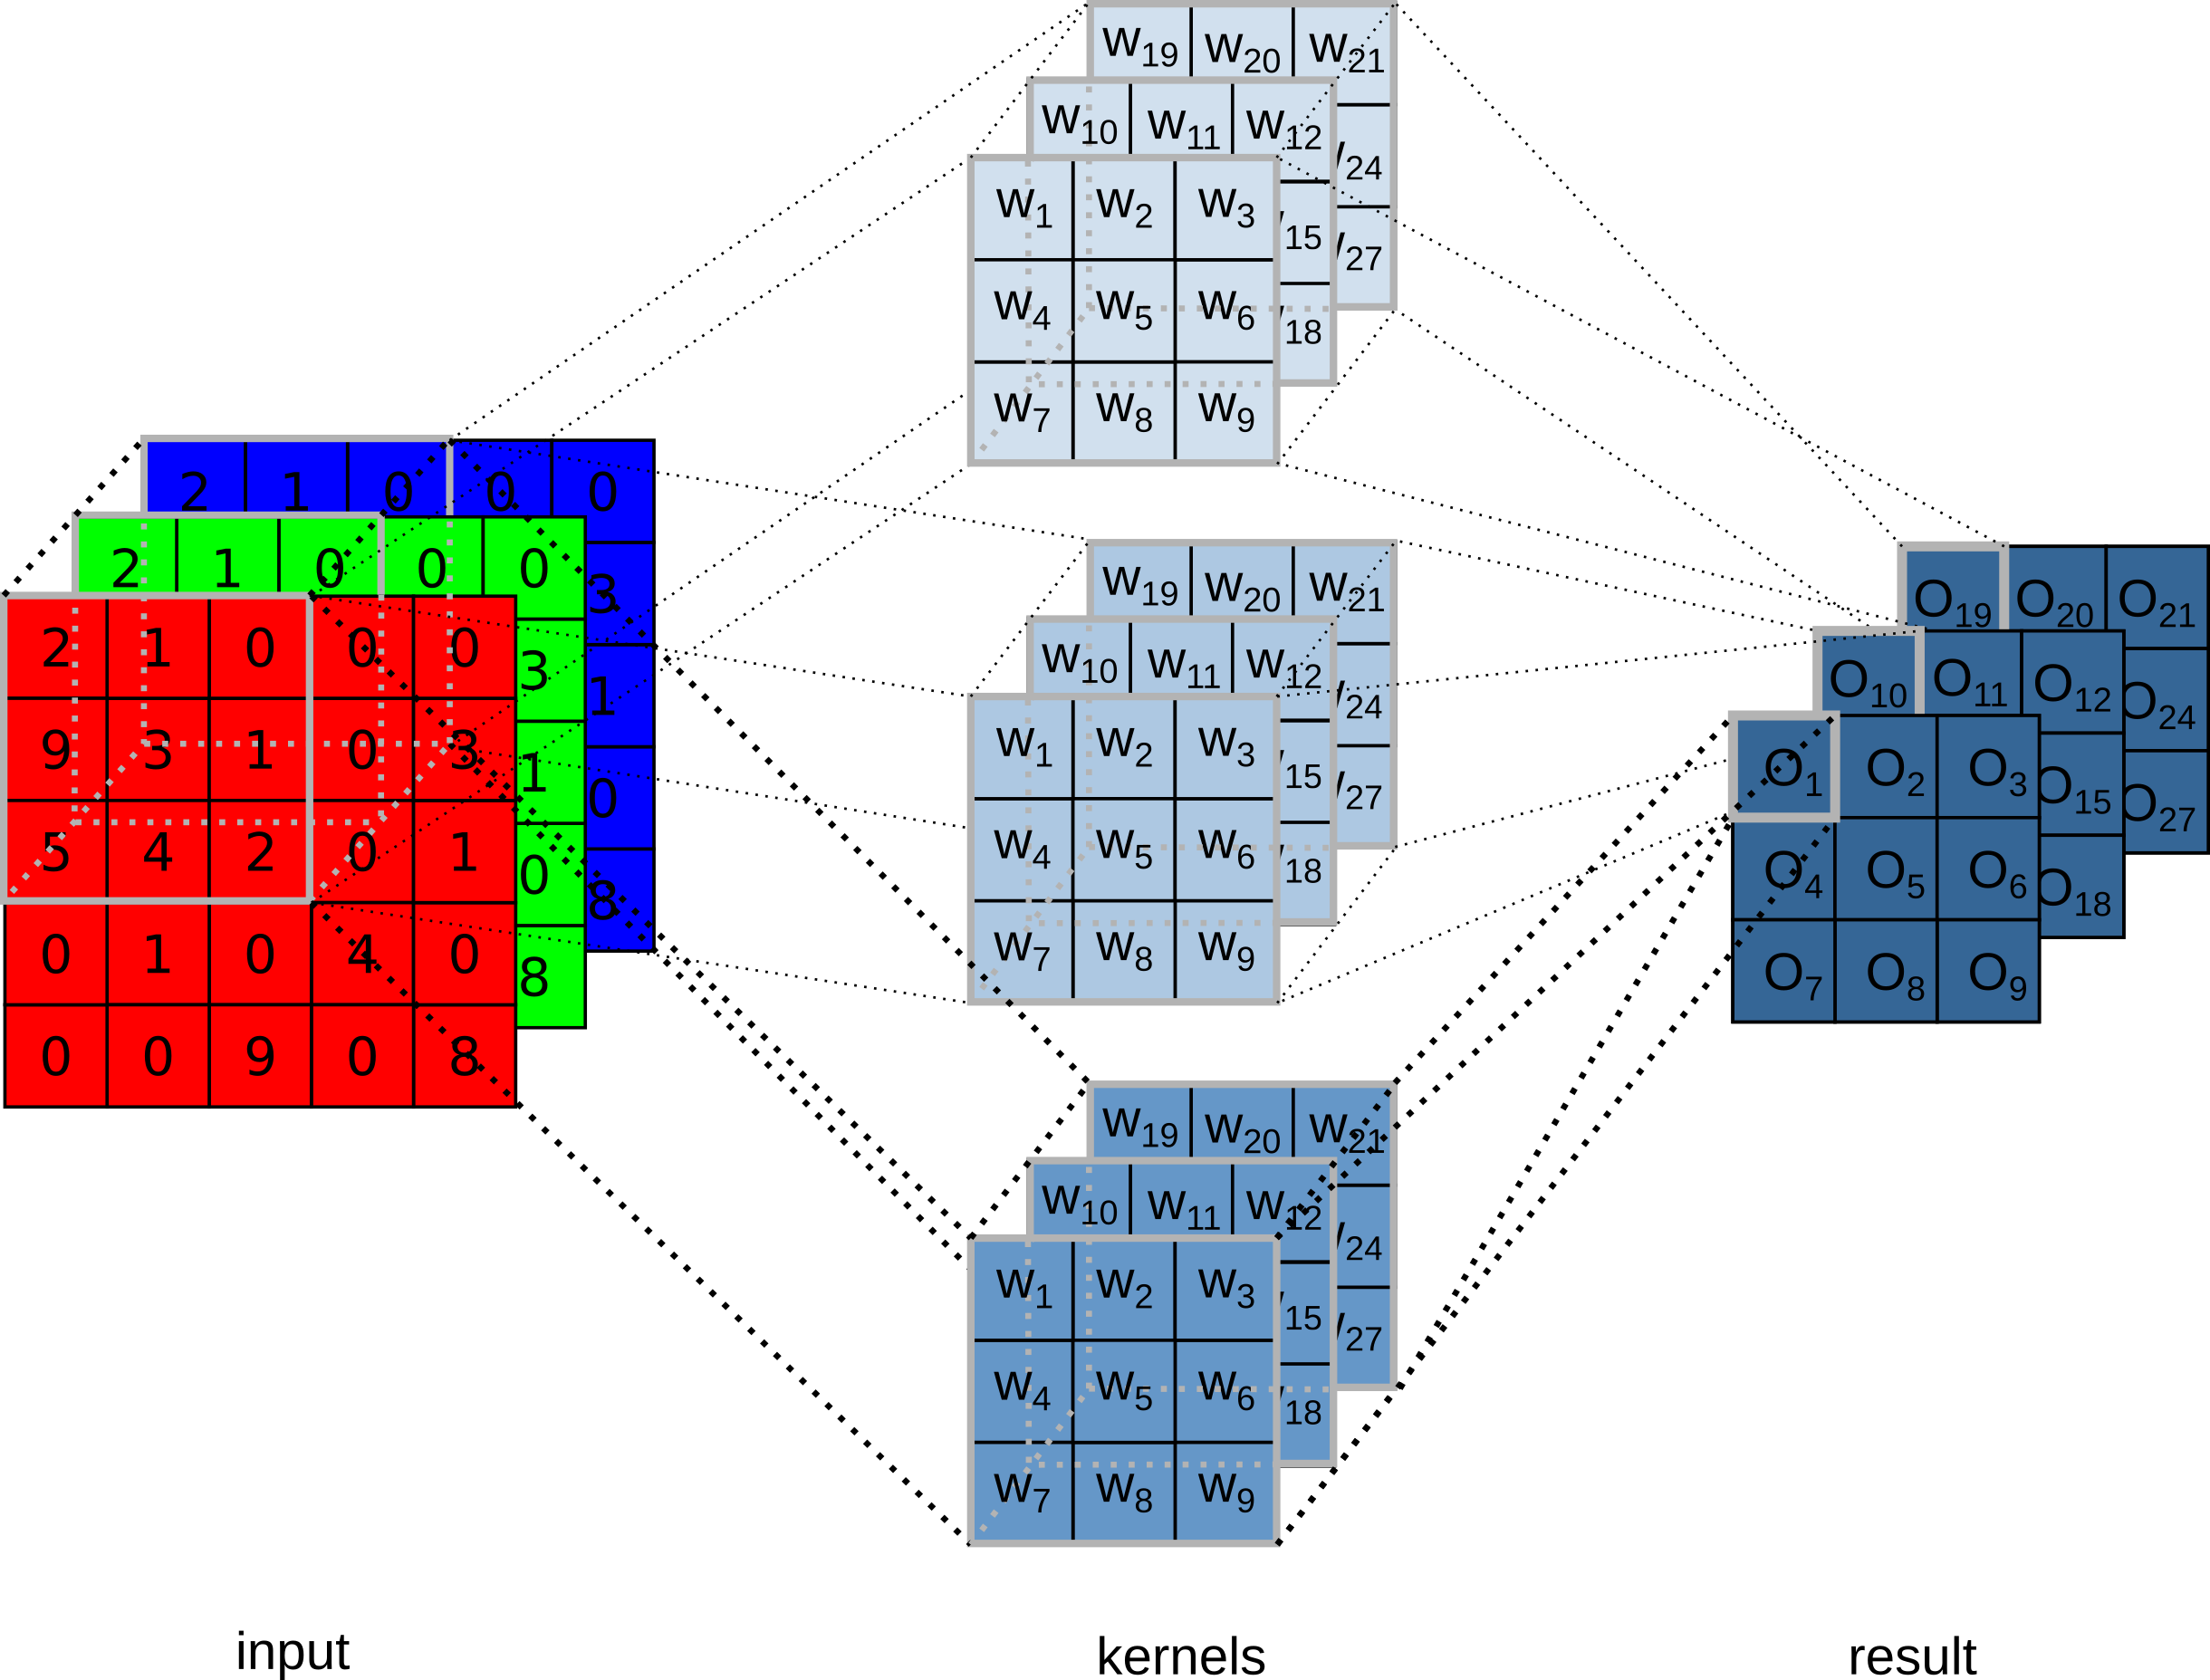
\includegraphics[scale=0.25]{"Part 3 - Learning Systems/Supervised Learning/Deep Learning/images/figure119.png"}
    \caption{Convolution of a 5x5x3 sized image with three 3x3x3 sized kernel and its result.}
    \label{fig:figure119}
\end{figure}

The two previous examples, Figures \ref{fig:figure117} and \ref{fig:figure119}, also serve to show us one of the features of convolution that makes it a good choice for working with images, what is called feature sparse iterations (also known as sparse connectivity) \cite{goodfellow2016}. This attribute highlights the fact that each output unit, or pixel, is connected to only a fraction of the input units. Figure \ref{fig:figure119} depicts another example where each output pixel is connected to a region of the 75 input pixels, through a 3x3x3 kernel. This is very useful, as our image can have millions of pixels, and by using smaller sized kernels, we will be able to detect small features such as edges, corners, etc \cite{goodfellow2016}. In the convolution layers, the values that the network must learn are the values present in the filters, so that way we will have few parameters to learn and store. Conversely, in a simple neural network, as we saw in the MLP chapter, an image at the input means that each pixel would be connected to each neuron in the next layer, thus resulting in an excessively large network.

Another important feature of CNNs is the ability to share the parameters, since the same filter is applied to different regions of the image using the same values, unlike a neural network without convolution layers, where we have a matrix with weights that are used for only one connection. The sharing of parameters gives us another feature, which is the invariance to translation , i.e., if we move the position of an object in the input image, its representation will also be moved in the resulting image \cite{goodfellow2016}.

\subsection{Padding}

In the convolution examples, Figures \ref{fig:figure117} and \ref{fig:figure119}, we see that as we apply the kernel to the input image, the size of the output image is reduced. In fact, by convolving a image of size $m \times n$ with a filter of size $k_m \times k_n$ the resulting image will have a height of $m-k_m+1$ and a length of $n-k_n+1$ . This type of convolution, where the resulting image is smaller, is often called “valid”.
If we want the output image to be the same size as the input image, we have to add more rows and columns to our image, this is known as padding. In this case, we use the formula  $m+2p-k_m+1$ and $n+2p-k_n+1$ where $p$ represents the padding. For example, in the previous Figures \ref{fig:figure117} and \ref{fig:figure119}, if the output has to be the same size as the input, we would have to use a padding of $6+2p-3+1=6p=1$.

\subsection{Stride}

The convolution examples we saw earlier used unitary steps. But we can also use larger steps, as this reduces the computational cost of performing these steps at intervals. This clearly has an impact on the resulting output, decreasing its resolution, but in cases where we do not need to extract delicate features this becomes a good option \cite{goodfellow2016}.

When we use a stride value greater than one, this will also affect the output size, which will be governed by the following relationship \cite{adrian2017}:

\begin{equation}
\frac{m+2p-k_m}{s}+1 \  \times \ \frac{n+2p-k_n}{s}+1
\end{equation}

Where $m$ and $n$ are the image dimensions, $p$ is the padding, $k_m$ and $k_n$ are the kernel dimensions and $s$ is the stride. Figure \ref{fig:stride} depicts an example with the steps of a convolution with s=2 using a kernel of size 3 over an image of size 5 x 5 and padding=0.

\begin{figure}
    \centering
    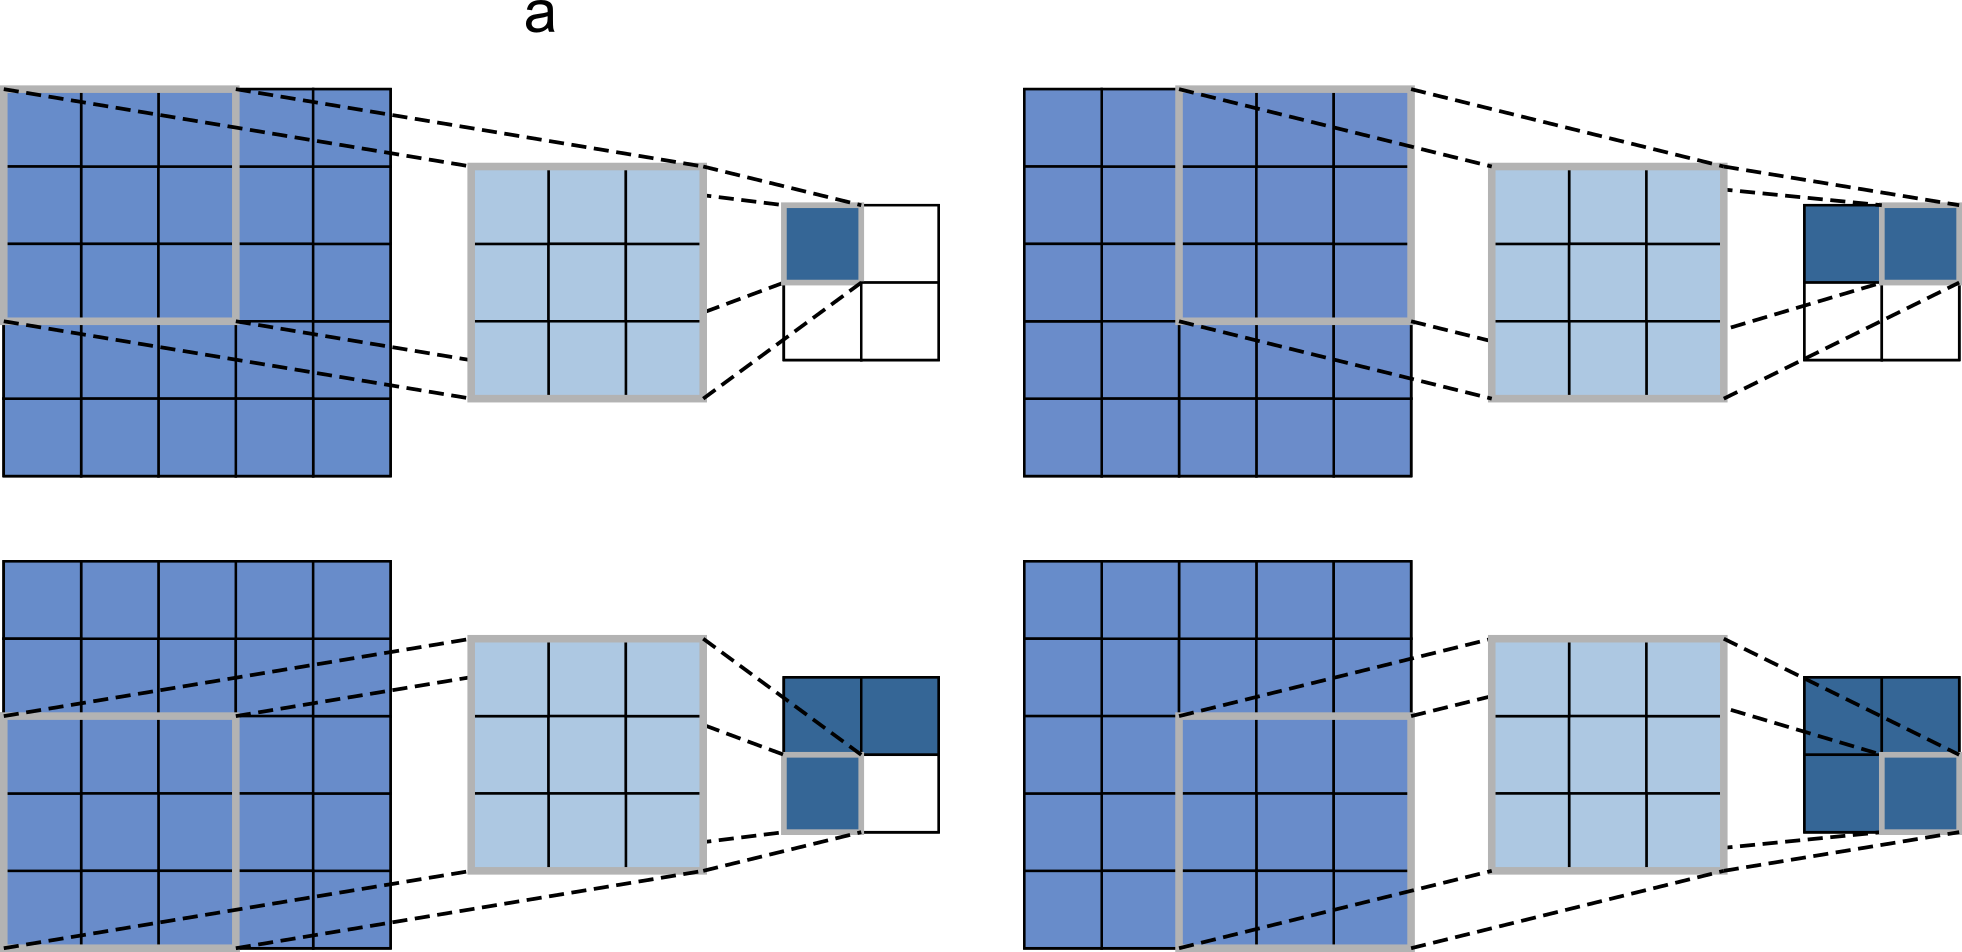
\includegraphics[scale=0.20]{"Part 3 - Learning Systems/Supervised Learning/Deep Learning/images/stride.png"}
    \caption{Example using a stride larger than 1.}
    \label{fig:stride}
\end{figure}

\subsection{Pooling Layer}

This is a very important layer, which aims to subsampling the image to reducing its size, and, consequently, reduce the total memory, processing and parameters needed, in addition to curbing the risk of overfitting \cite{geron2019}\cite{adrian2017}\cite{elgendy2020}.

As in convolution layers each output unit is connected to an input region, we must also take into account the size of the kernel, stride and padding. But, unlike the convolution, the “kernel,” or, in other words, the region that will connect us to the input, will have no weights, it will perform only one operation, the most common being the maximum or the average \cite{geron2019} .

Figure \ref{fig:figure121} depicts an example of max pooling, where we can see how it works(Figures \ref{fig:figure121}(a-d)). This example uses a region of 2 x 2 , which is very common \cite{adrian2017}, and stride=1.

\begin{figure}
    \centering
    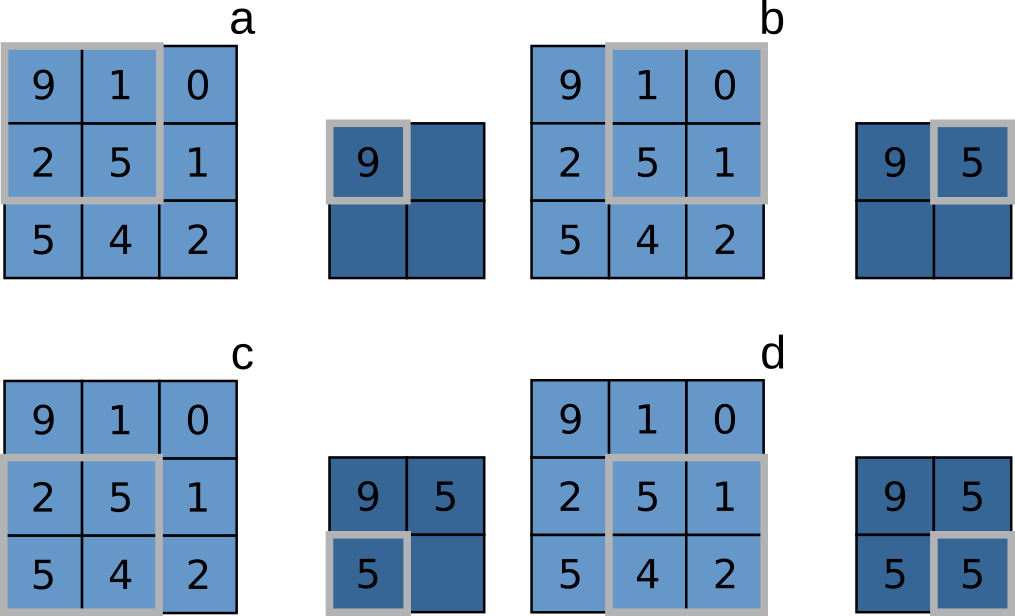
\includegraphics[scale=0.30]{"Part 3 - Learning Systems/Supervised Learning/Deep Learning/images/figure121.png"}
    \caption{Example of max pooling application.}
    \label{fig:figure121}
\end{figure}

Figure \ref{fig:figure122} depicts another example of max pooling, but this time performed with a larger input, we can see that the operation is performed on each input layer of the object, and that its output contains the same number of layers as the input, which is what typically occurs in this type of operation \cite{geron2019}.

\begin{figure}
    \centering
    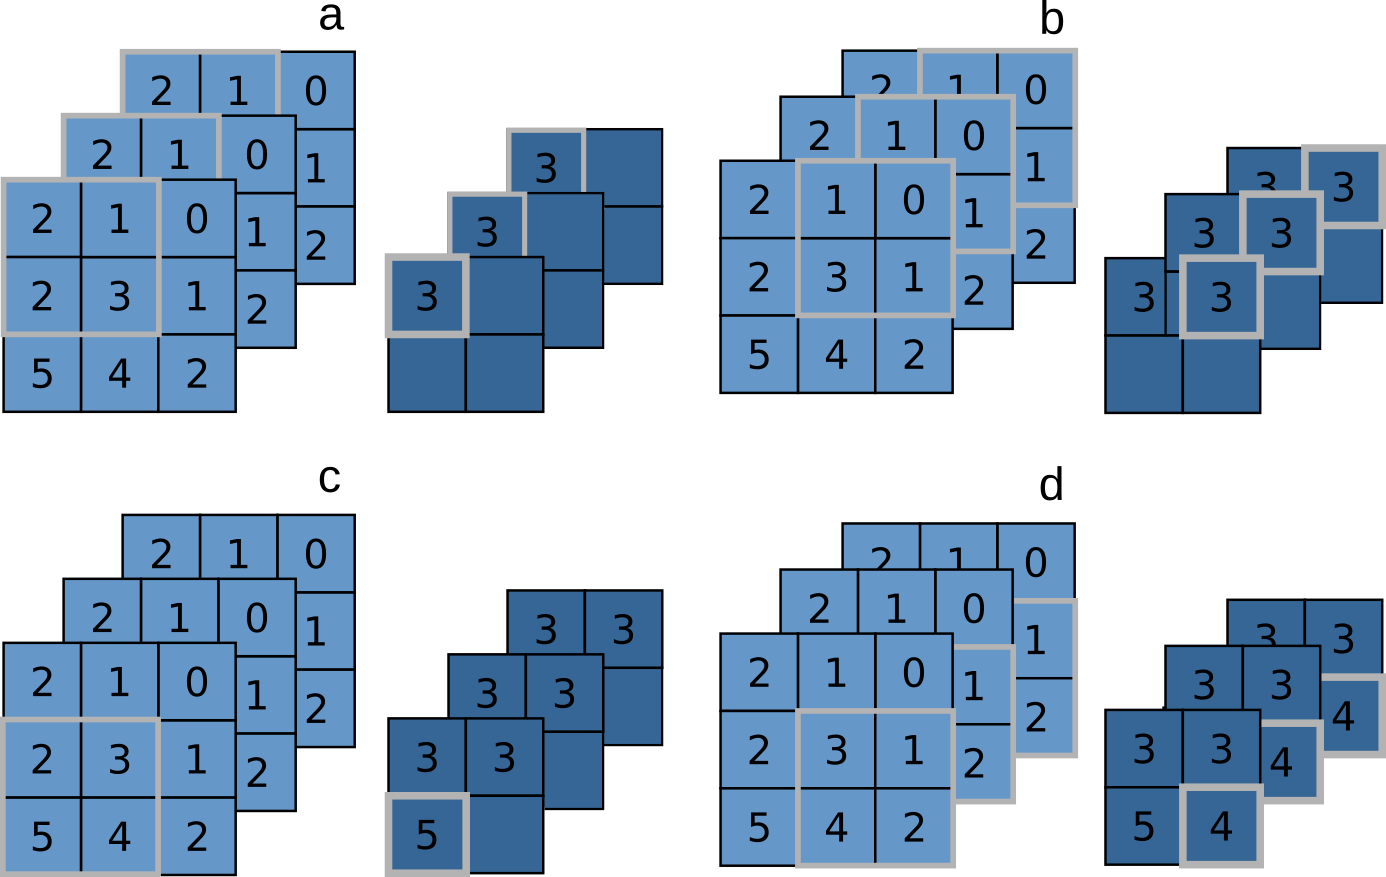
\includegraphics[scale=0.30]{"Part 3 - Learning Systems/Supervised Learning/Deep Learning/images/figure122.png"}
    \caption{Example of max pooling application in an image with more dimensions.}
    \label{fig:figure122}
\end{figure}

Although pooling is a very popular technique, we can find scientific works where their authors preferred not to use pooling to perform subsampling, but to use convolution layers with higher stride and padding values to achieve dimension reduction \cite{elgendy2020}\cite{adrian2017}. This way of working was proposed by Springenberg \cite{springenberg2014striving}, where they demonstrate that even networks without pooling layers can yield good results for different databases, such as CIFAR-10 and ImageNet.

\subsection{Fully Connected Layers}

CNNs usually have several convolution layers followed by activation functions, which in turn are followed by pooling layers, and this process decreases the dimensions $m \times n$ and increases the depth of the CNN model, that is, the number of feature layers (known as feature maps ) \cite{elgendy2020}\cite{geron2019}. Figure \ref{fig:figure123} depicts a representation of this process through the network topology. At the end of this network we have a large amount of layers with the characteristics extracted from the input image, and we need to use this information. In this same Figure, we can see that in the end we have fully connected layers, which is a regular neural network, an MLP \cite{elgendy2020}.

\begin{figure}
    \centering
    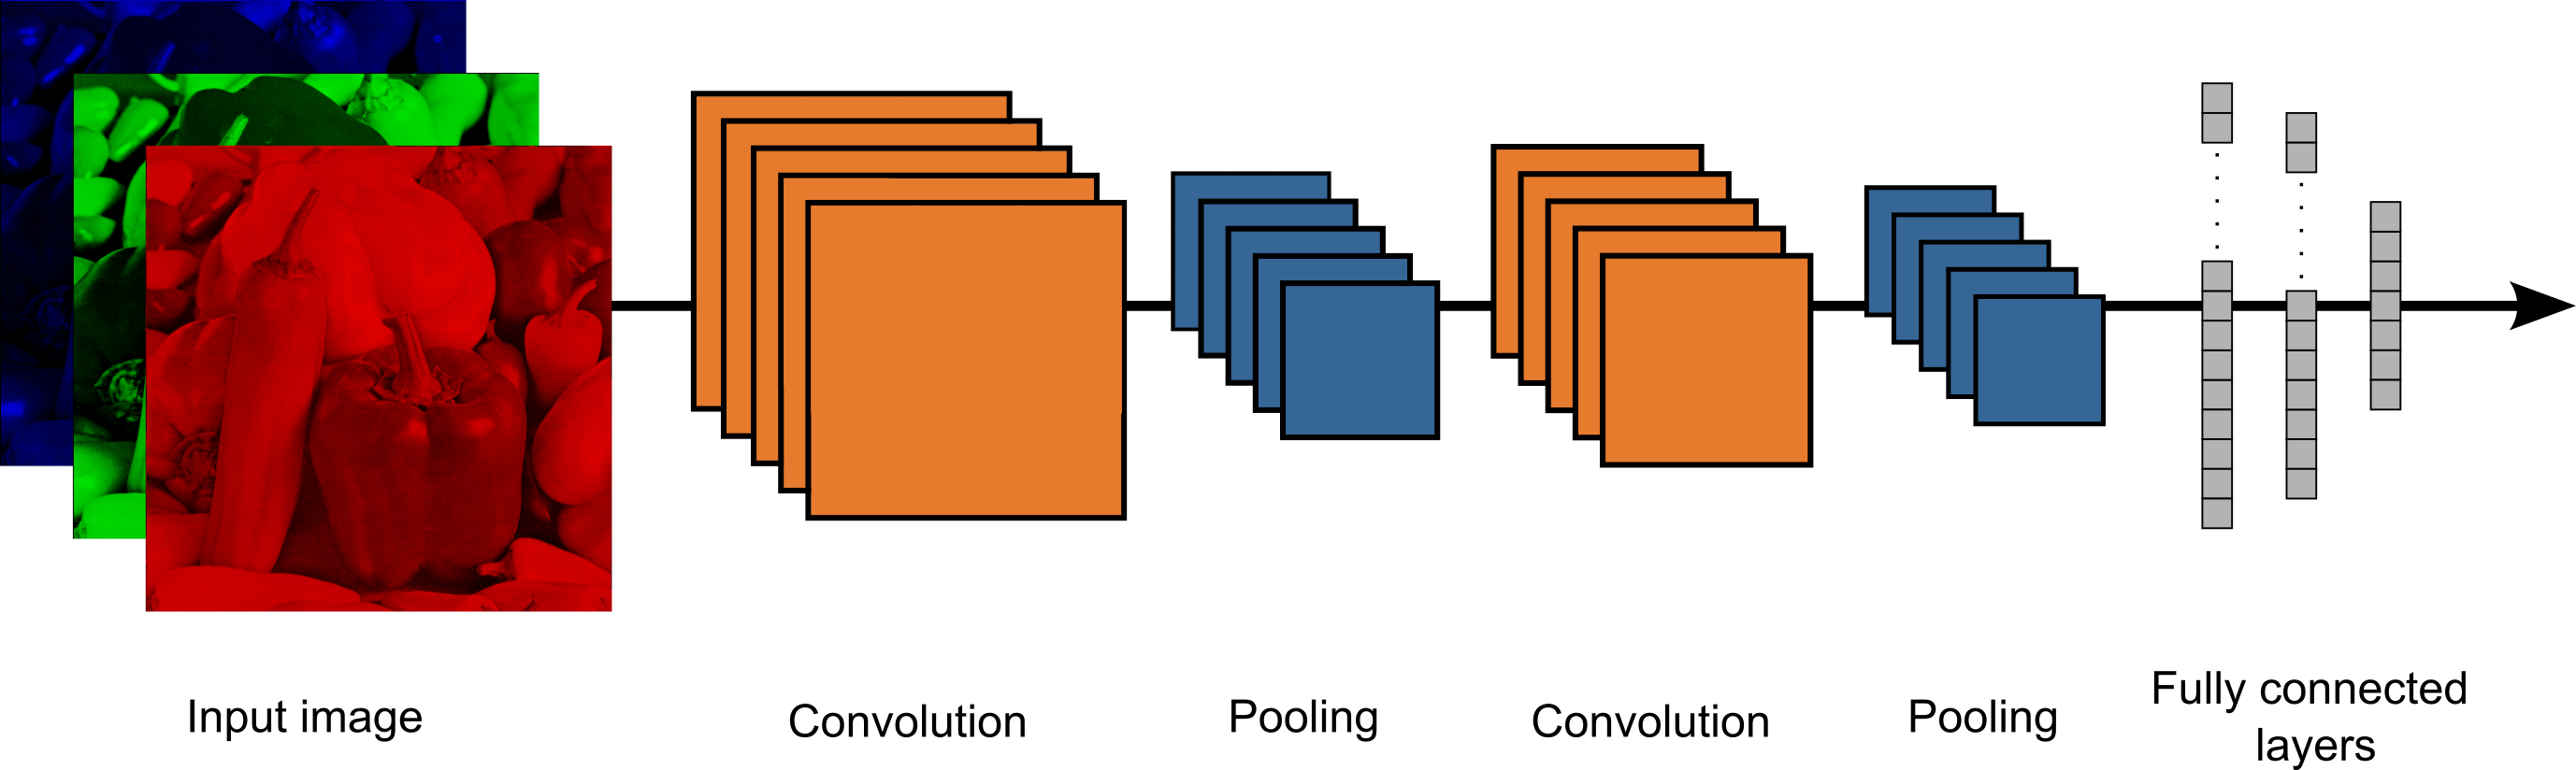
\includegraphics[scale=0.22]{"Part 3 - Learning Systems/Supervised Learning/Deep Learning/images/figure123.png"}
    \caption{Example of max pooling application  in an image with more dimensions.}
    \label{fig:figure123}
\end{figure}

Figure \ref{fig:figure124} depicts the representation of the use of the information extracted from the image by the convolution layers. In this example, the data ends with a size of 7x7x64, that is, we have 64 feature maps with a size of 7x7. To provide this data to the full connected layer, we have to flatten these feature maps to a vector of dimensions 1x3136, that passes through the network and ends in the layer of Softmax, resulting in the output vector.

\begin{figure}
    \centering
    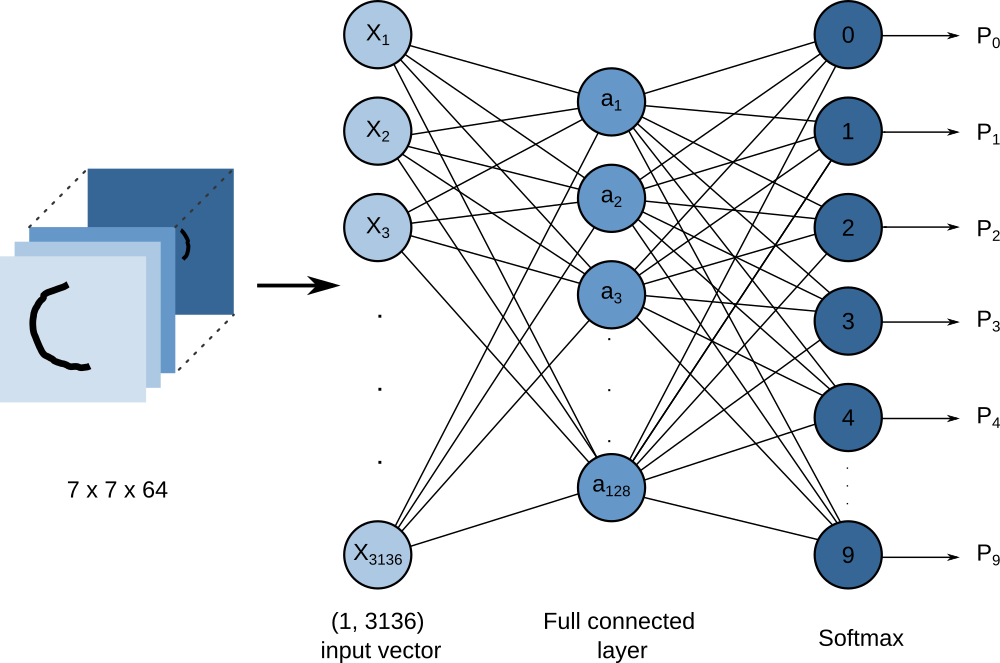
\includegraphics[scale=0.50]{"Part 3 - Learning Systems/Supervised Learning/Deep Learning/images/figure124.png"}
    \caption{Example of fully connected layers application in an image with more dimensions.}
    \label{fig:figure124}
\end{figure}

